\chapter{مروری بر مفاهیم مورد نیاز}
\section{تبدیلات سیگنال صوتی}
یک اجرای موسیقی می‌تواند کاملا توسط تغییرات ایجاد شده در فشار هوا طی زمان توصیف
شود. این نمایش به صورت سنتی محور افقی نماینده زمان است و محور عمودی نماینده
تغییرات ایجاد شده در فشار یا شدت سیگنال است. با توجه به این که کامپیوترها
توانایی پردازش اطلاعت پیوسته را ندارند، این سیگنال‌ها نیاز دارند تا گسسته‌سازی
شوند. با توجه به این گوش انسان می‌تواند اصواتی با فرکانس تا ۲۰ کیلوهرتز را بشنود
و پردازش کند، برای این که تمام اطلاعات مورد نیاز بتواند ذخیره شود، نمونه برداری
با حداقل دقت ۴۰ کیلوهرتز انجام شود. به صورت رایج موسیقی معمولا در ۴۴/۱ کیلوهرتز
نمونه برداری می‌شود. همچنین برای ذخیره هر نمونه از ۱۶ بیت استفاده می‌شود.
فایل‌های wav از این نمایش برای ذخیره سازی موسیقی استفاده می‌کنند.

هر چند که صوت تنها حاصل نوسانات ماده است، ولی سیستم شنوایی این نوسانات به
مجموعه‌ای از فرکانس‌ها تبدیل می‌شود و سپس پردازش می‌شوند. برای تشخیص میزان وجود
یک فرکانس خاص در یک سیگنال صوتی می‌توان همبستگی سیگنال صوتی را با یک سیگنال
سینوسی در فرکانس خواسته شده را محاسبه کرد. هرچند دو سیگنال سینوسی با فرکانس
یک‌سان نیز می‌توانند همبستگی صفر داشته باشند اگر فاز آن‌ها به میزان مناسبی با هم
اختلاف داشته باشد. این موضوع به خوبی در شکل زیر نشان داده شده است.
\begin{figure}[ht]
    \centering
    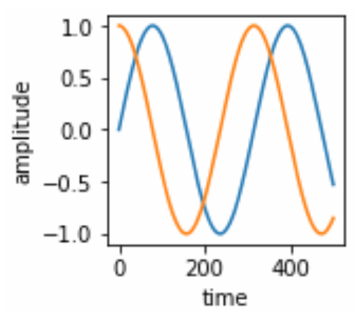
\includegraphics[height=5cm]{./statics/uncorrelated_sine_waves.png}
    \caption{دو سیگنال سینوسی که با هم وابستگی ندارند ولی هر دو در فرکانس یکسانی نوسان می‌کنند}
\end{figure}

برای اندازگیری همبستگی به ازای تمام فازهای ممکن، مانند فازی که باعث می‌شود تا
مقدار همبستگی حداکثر شود، از اعداد موهومی استفاده می‌شود. فرض کنید نقطه‌ای برروی
محور اعداد موهومی از مبدا و در جهت اعداد حقیقی مثبت شروع به حرکت کند. جهت حرکت
این نقطه با با توجه به فرکانس خواسته شده تغییر می‌کنند. همچنین سرعت حرکت این
نقطه در لحظه $t$ برابر با قدرت سیگنال ورودی در  لحظه $t$ است. به عبارتی دیگر،
نقطه یاد شده در زمان $t$ به اندازه قدرت سیگنال ورودی در زمان $t$ و در جهت محاسبه
شده جابه‌جا می‌شود. در پایان فرآیند هرچه نقطه از مبدا دورتر شده باشد، یعنی
وابستگی سیگنال ورودی با سیگنالی سینوسی با فرکانسی برابر فرکانس خواسته شده بیشتر
است. همچنین فازی که باعث بیشتر مقدار وابستگی می‌شود، با جهت کلی حرکت در ارتباط
هست. شکل زیر نمونه‌ای از انجام این فرآیند را برای دو سیگنال مختلف نشان می‌دهد.
مطابق انتظار برای سیگنالی که هم بستگی بسیار پایینی با فرکانس خواسته شده دارد،
نقطه نزدیک مبدا است و برای سیگنالی که همبستگی بیشتری دارد، از مبدا دورتر است.
\begin{figure}[ht]
    \centering
    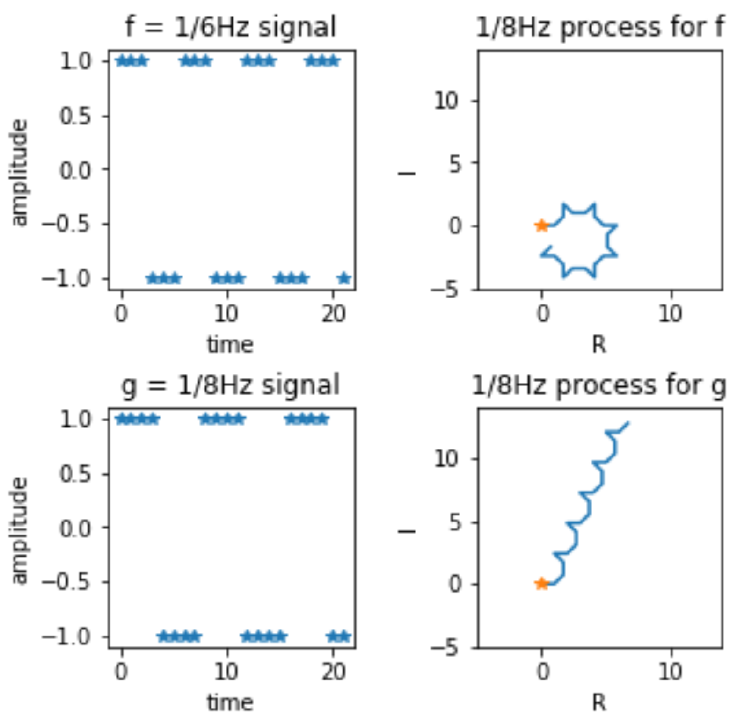
\includegraphics[height=8cm]{./statics/spectral_domain_process.png}
    \caption{انجام فرایند توضیح داده شد بر روی دو سیگنال ورودی مختلف}
\end{figure}

فرایند بالا را می‌توان توسط رابطه زیر مدل کرد:
\begin{equation}
    X(\omega) = \sum_{n} x(n)e^{i \omega \frac{2\pi}{f_s} n}
\end{equation}
که $X(\omega)$ عددی موهومی است که اندازه آن برابر است با میزان حضور یک فرکانس
دلخواه مانند $\omega$ در سیگنال ورودی $x$. همچنین $x(n)$ میزان قدرت سیگنال در در
نمونه $n$ نشان می‌دهد. $e^{i \omega \frac{2\pi}{f_s}}$ برابر جهت حرکت در محور‌
مختصات اعداد موهومی در زمان $t = \frac{n}{f_s}$ است که $f_s$ فرکانس خواسته شد
است. محل توقف نقطه در فرآیند یاد شده همان خروجی این رابطه است که اندازه آن با
میزان حضور فرکانس مطلوب در سیگنال ورودی رابطه دارد.

با کمک رابطه بالا می‌توان می‌توان میزان وجود هر فرکانس در سیگنال ورودی را اندازه
گرفت و در نتیجه سیگنال ورودی را به حوزه فرکانس انتقال داد. حوزه فرکانس میزان
قدرت هر فرکانس در سیگنال ورودی را بیان می‌کند در حالی که حوزه زمان که ابتدا سیگنال
در آن بود قدرت سیگنال در زمان‌های مختلف را مشخص می‌کند.

\subsection{تبدیل فوریه}
معروف‌ترین تبدیل برای انتقال سیگنال از حوزه زمان به حوزه فرکانس تبدیل فرویه هست.
\gls{fft} یک پیاده سازی از این تبدیل است که سیگنال‌هایی که طول آن‌ها توانی از دو
است را می‌توان در $O(nlog(n))$ به حوزه فرکانس ببرد. این تبدیل میزان فعال بودن
فرکانس‌های مختلف را که فاصله خطی از هم دارند را به گونه‌ای محاسبه می‌کند که
سیگنال ابتدایی مجدد بعد از تبدیل قابل محاسبه است. این تبدیل سیگنال ورودی را به
شکل حاصل جمع مجموعه‌ای موج سینوسی با فرکانس‌های مختلف بیان می‌کند. صورت گسسته
این تبدیل که به \gls{dft} معروف است توسط رابطه زیر قابل محاسبه است:
\begin{equation}
    X[k] = \sum_{n=0}^{N-1} x[n]e^{- ikw\omega_0n} \quad \forall k \in \{ 0, 1, ..., N-1 \}
\end{equation}
که $x$ سیگنال ورودی به طول $N$ است و $\omega_0$ برابر $\frac{2\pi}{n}$ است.

همچنین برای بازتولید سیگنال اولیه می‌توان از رابطه زیر استفاده کرد:
\begin{equation}
    x[n] = \frac{1}{N}\sum_{k=0}^{N-1} X[k]e^{ik\omega_0n} \quad \forall n \in \{ 0, 1, ..., N-1 \}
\end{equation}

به صورتی کلی وقتی خروجی تبدیل بررسی می‌شوند تنها اندازه اعداد موهومی به دست آمده
استفاده می‌شود. اندازه این اعداد متناسب با همبستگی سیگنال ورودی با سیگنال‌های
سینوسی بهینه است.

با توجه به سرعت \gls{fft} این تبدیل از حوزه‌های متفاوت به صورت گسترده استفاده
می‌شود. با این وجود در حوزه \gls{mir} این تبدیل یک ضعف مهم دارد. به کمک این
تبدیل می‌توان متوجه شد که یک فرکانس خاص، مثلا ۴۴۰ هرتز، در یک قطعه وجود دارد ولی
راهی برای تشخیص مکان وجود این فرکانس وجود ندارد. یک راه حل برای این ضعف این است
که سیگنال ورودی در فواصل کوتاه برش داده شود و برای هر برش به صورت جداگانه تبدیل
محاسبه گردد. این تبدیل جدید به \gls{stft} معروف است. هرچی فاصله زمانی که برش‌ها
در آن‌ها انجام می‌شود کوتاه‌تر باشد، دقت خروجی در بعد زمان بیشتر است. از طرفی
دیگر کوتاه بودن این فواصل زمانی باعث کاهش دقت در بعد فرکانس می‌شود. خروجی
\gls{STFT} یک نمایش دو بعدی است که یک محور آن نماینده زمان و محور دیگر نماینده
فرکانس است. این نمایش به نمایش زمان-فرکانس معروف است.

\subsection{تبدیل ثابت Q}
یکی از ضعف‌های \gls{stft} در حوزه موسیقی این است که فرکانس‌هایی که وجود آن‌ها در
سیگنال ورودی بررسی می‌شود، فاصله خطی از یک دیگر دارند. این در حالی هست که
\gls{pitch} نت‌های موسیقی در فواصل لگاریتمی از یک دیگر قرار دارند. این تفاوت‌ به
این معنی است که برای نت‌های بم تعداد زیادی فرکانس وجود دارد ولی برای نت‌های
زیرتر فرکانس‌های کمتری وجود دارد.

\gls{cqt} بجای استفاده از فواصل خطی از فواصل لگاریتمی استفاده می‌کند. ایده اصلی
این است که در فرایند توضیح داده شده در ابتدا، فرکانس‌های انتخابی، فاصله‌ای
لگاریتمی نسبت به هم داشته باشند. همچنین این تبدیل به کمک توابع پنجره‌بندی تنها
در بازه‌های زمانی خاصی، وجود فرکانس‌ها را بررسی می‌کند.
\begin{figure}
    \centering
    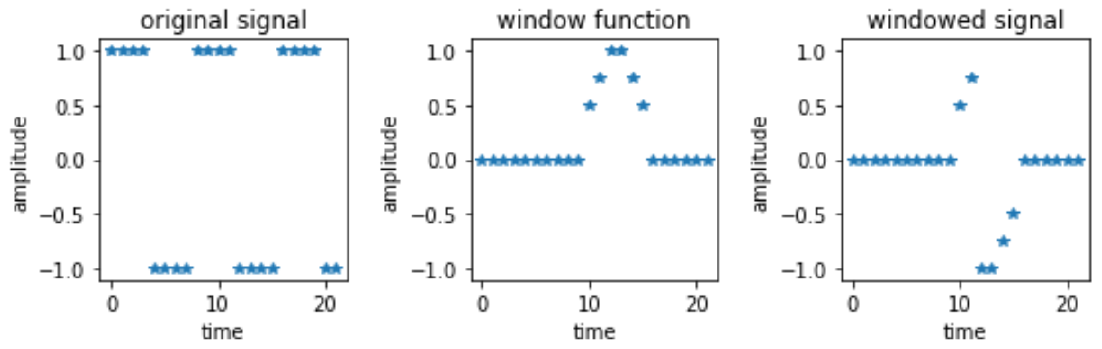
\includegraphics[height=4cm]{./statics/windowed_signal.png}
    \caption{نمونه‌ای از یک سیگنال پنجره‌بندی شده}
\end{figure}

\gls{CQT} را می‌توان به کمک رابطه زیر محاسبه کرد:
\begin{equation}
    X^{CQ}(k, n) = \sum_{j=n-\lfloor N_k / 2 \rfloor}^{n+\lfloor N_k / 2 \rfloor} x(j)a_k^*(j-n+N_k/2) \quad \forall k \in \{1, 2, ..., K \}
\end{equation}
\begin{equation}
    a_k^*(n) = \frac{1}{N_k} w (\frac{n}{N_k}) e^{if_k\frac{2\pi}{f_s}n}
\end{equation}
$X^{CQ}(k, n)$ مقدار خروجی تبدیل برای فرکانس $f_k$ و در اطراف نمونه $n$ سیگنال
ورودی $x$ است. $N_k$ یک عدد حقیقی هست که از پارامترهای تبدیل است. $w$ یک تابع
پنجره‌بندی پیوسته هست که دامنه آن بین صفر و یک است. $f_k$ فرکانس خواسته شده‌
$k$ام است. $f_s$ نیز فرکانسی است که سیگنال ورودی با آن نمونه برداری شده است.

این تبدیل پارامترهای مختلفی دارد که مقدار بهینه آن‌ها با توجه به معیار‌هایی
مانند توانایی باز تولید سیگنال و سرعت محاسبه در \cite{schorkhuber2010constant}
بررسی شده است. در ادامه به بررسی این پارامترها می‌پردازیم.

$f_k$ مقدار فرکانس $k$ام خواسته شده را مشخص می‌کند. با توجه به این که این
فرکانس‌ها با هم فاصله‌ای لگاریتمی دارند، می‌توان مقدار آن‌ها را مقایسه کرد. برای
محاسبه می‌توان از رابطه زیر استفاده کرد:
\begin{equation}
    f_k = f_1 2^{\frac{k-1}{B}} \quad \forall k \in \{1, 2, ..., K\}
\end{equation}
$f_1$ یا $f_{min}$ مقدار پایین‌ترین فرکانس را مشخص می‌کند که سایر فرکانس‌ها از
آن شروع می‌شوند. $B$ مشخص می‌کند به ازای هر اکتاو چند فرکانس انتخاب شود و میزان
حضور آن‌ها در سیگنال ورودی اندازه گرفته شود. همچنین $K$ تعداد کل فرکانس‌های
خواسته شده است. این مقدارها با توجه کاربرد به می‌توانند انتخاب شوند.

$N_k$ عرض پنجره استفاده شده برای فرکانس $k$ام را مشخص می‌کند. مقدار بهینه این
پارامتر را می‌توان با استفاده از رابطه زیر محاسبه کرد:
\begin{equation}
    N_k = \frac{qf_s}{f_k(2^{\frac{1}{b}}-1)} \stackrel{B \geq 12}{\approx} \frac{qf_sB}{log(2)f_k} \quad 0 < q \leq 1
\end{equation}

انجام \gls{cqt} برای هر نمونه نه از نظر محاسبه منطقی است و نه مزیت خاصی دارد. از
این جهت این تبدیل به ازای هر $H_k$ نمونه یک بار انجام می‌شود. مقدار بهینه برای
این پارامتر برابر $\lfloor \frac{1}{2N_k} \rfloor$ است تا تمام طول سیگنال ورودی
پردازش شود. همچنین در عمل معمولا به ازای تمام مقادیر $k$، $H_k = H$ است تا خروجی
را بتوان به شکل یک ماتریس نمایش داد.

$w$ تابع پنجره‌بندی مورد استفاده است که به صورت سنتی از تابع $Hann$ برای آن
استفاده می‌شود. این تابع برشی از تابع سینوس‌ هست که در زیر نمودار آن نشان داده شده
است.
\begin{figure}[ht]
    \centering
    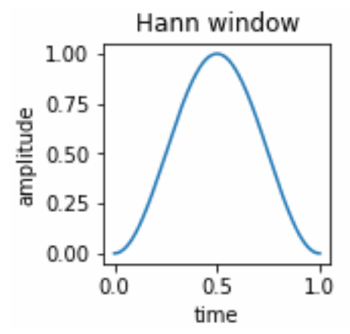
\includegraphics[height=5cm]{./statics/hann_plot.png}
    \caption{نمودار تابع پنجره‌بندی Hann}
\end{figure}

در نهایت $f_s$ فرکانس نمونه‌برداری از سیگنال اولیه است. برای صحت محاسبات رابطه
زیر باید برقرار باشد:
\begin{equation}
    f_s \geq 2f_k
\end{equation}

\subsection{اسپکتروگرام mel}
با توجه به این که درک انسان از صوت یک درک کاملا لگاریتمی نیست، مقیاس دیگری برای
انجام آزمایشات ساخته شده است که به مقیاس mel معروف است. با وجود این که بیش از یک
مقیاس mel ساخته شده، ولی تمام آن‌ها تنها تفاوت‌هایی جزئی با هم دارند. در این
پایان‌نامه فقط یکی از این مقیاس‌ها توضیح داده شده است که همان مقیاسی است که در
این پایان‌نامه استفاده شده است و کتابخانه librosa آن را پیاده‌سازی کرده است
\cite{mcfee2015librosa}.

آزمایشات انجام شده بر روی شنوایی انسان نشان داده‌اند که درک انسان از صوت، تا
هزار هرتز، یک درک خطی است. برای اصوات بالای هزار هرتز این درک به شکل لگاریتمی در
می‌آید. با این توصیف رابطه زیر می‌تواند این مقیاس را مدل کند:
\begin{equation}
    x Hz =
    \begin{cases}
        \frac{3x}{200}mel &\quad x \leq 1000\\
        15 + 27 ln(x/1000) / ln(6.4) mel &\quad \text{elsewhere}
    \end{cases}
\end{equation}

کتاب‌خانه librosa \gls{spec} با مقیاس mel را به کمک رابطه زیر محاسبه می‌کند:
\begin{equation}
    X^{MEL}(k, n) = \sum_{j=0}^{n_{fft}-1} |X_n|^2(j)A_k^*(\frac{f_s}{n_{fft}}j)
\end{equation}
$|X_n|$ اندازه \gls{dft} سیگنال ورودی $x$ در اطراف $n$ با $n_{fft}$ نمونه است.
$A_k^*$ یک تابع پنجره‌بندی از اعداد حقیقی به اعداد حقیقی است. این تابع شکلی
مثلثی دارد و در $f_{k-1}$ مقدار صفر دارد. در $f_k$ به $V_{max}^{k}$ می‌رسد و
مجددا در $f_{k+1}$ صفر می‌شود. $V_{max}^{k}$ به گونه‌ای مقدار داده می‌شود که
تقریبا برای هر کانال مقداری ثابت داشته باشد. این مقدار از رابطه زیر به دست
می‌آید:
\begin{equation}
    V_{max}^{k} = \frac{2}{f_{k+1} - f_{k-1}}
\end{equation}
$\frac{f_s}{n_{fft}}j$ فرکانس متناظر با $j$امین فرکانس استفاده شده در \gls{dft}
است. همچنین $f_s$ فرکانس نمونه‌گیری سیگنال ورودی $x$ است.

\subsection{قالب فرکانسی یک نت}
وقتی که صوت حاصل از اجرای یک نت تنها، از حوزه زمان به خوزه فرکانس انتقال داده
شود، \gls{spec} به دست آمده، قالب فرکانس آن نت نامیده می‌شود. وقتی که

در شکل زیر قالب فرکانسی نت $A5$ که بر روی ساز پیانو اجرا شده است رسم شده است.
همچنین فرکانس‌ها با یک دیگر فاصله‌ای لگاریتمی دارند تا متناظر با \gls{pitch}
نت‌های پیانو باشند. همچنین که در \gls{spec} رسم شده کاملا واضح است، علاوه بر
فرکانس پایه نت، فرکانس‌های پایه‌ای دیگری نیز کامل در صوت تولید شده حضور دارند.
این فرکانس‌ها با خط سفید مشخص شده‌اند. این پدیده رفتاری کاملا انتظار از یک ساز
موسیقی است و یکی از عوامل اصلی سختی مسئله \gls{atm} محسوب می‌شود. همچنین این
رفتار وجه اصلی تمایز مسئله \gls{asr} با مسئله \gls{atm} است. این فرکانس‌‌های
فعال، به عنوان هامونیک‌های نت نواخته شده شناخته می‌شود. با توجه به این که این
هامونیک‌ها خود متناظر با نت‌های دیگری نیز هستند که احتمال نواخته شدن بالایی نیز
با نت پایه دارند، تشخیص نت‌های فعال را بسیار پیچیده می‌کنند.

همچنین، با توجه به شکل کاملا واضح است که در لظحه نواخته شدن نت، فرکانس‌های فعال
دیگری نیز در صوت تولید شده حضور دارند. دلیل حضور این فرکانس‌ها این است که وقتی
یک سیم پیانو توسط چکش نواخته می‌شود، در لحظه شروع حجم زیادی نویز تولید می‌کند که
باعث حضور بازه گسترده‌ای از فرکانس‌ها می‌شود. ولی پس از گذشت زمانی کوتاه، سیم
شروع می‌کند به در فرکانس متناظر نوسان کردن و فرکانس‌های اضافه حذف می‌شوند. حضور
این بازه گسترده از فرکانس‌ها باعث می‌شود که شروع نت‌ها به شکل بسیار ساده‌تری
قابل تشخیص باشد.
\begin{figure}[ht]
    \centering
    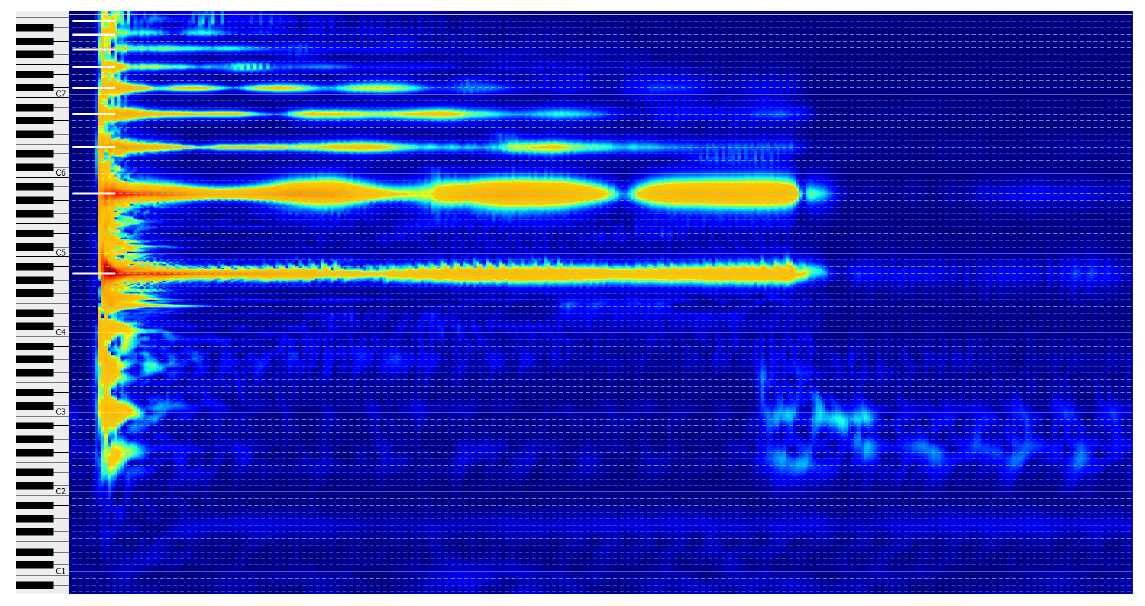
\includegraphics[width=15cm]{./statics/a5_spec.png}
    \caption{\gls{spec} متناظر با نواخته شدن نت A5 بر روی پیانو}
\end{figure}